\documentclass[aspectratio=169,10pt]{beamer}
\usetheme{Madrid}
\usecolortheme{default}
\setbeamertemplate{navigation symbols}{}
\setbeamertemplate{footline}[frame number]
\usepackage{amsmath,amssymb,booktabs,mathtools,graphicx,hyperref,xcolor,array}
\newcolumntype{P}[1]{>{\raggedright\arraybackslash}p{#1}}
\usepackage{xeCJK}
\setCJKmainfont{Heiti SC}
\setCJKsansfont{Heiti SC}
\setmainfont{Helvetica Neue}
\setsansfont{Helvetica Neue}
\definecolor{navy}{HTML}{003366}\definecolor{sbred}{HTML}{CC0000}\definecolor{sbblue}{HTML}{0066CC}
\definecolor{positive}{HTML}{0173B2}\definecolor{negative}{HTML}{DE8F05}\definecolor{emphasis}{HTML}{029E73}\definecolor{neutral}{gray}{0.55}
\newcommand{\pos}[1]{\textcolor{positive}{#1}}\newcommand{\con}[1]{\textcolor{negative}{#1}}\newcommand{\HL}[1]{\textcolor{emphasis}{#1}}\newcommand{\new}[1]{\textcolor{sbred}{#1}}
\setbeamercolor{structure}{fg=navy}
\setbeamercolor{palette primary}{bg=navy,fg=white}\setbeamercolor{palette secondary}{bg=sbblue,fg=white}\setbeamercolor{palette tertiary}{bg=navy!80!black,fg=white}
\setbeamercolor{title}{bg=navy,fg=white}\setbeamercolor{frametitle}{bg=navy,fg=white}
\setbeamerfont{frametitle}{size=\large,series=\bfseries}
\title[Awesome Schrödinger Bridge]{Awesome Schrödinger Bridge}
\subtitle{从经典 SB 到 2026：求解器、控制、离散与具身应用 —— 仓库交付与趋势汇报}
\author{Presenter: Yufeng Li (asimfish)}
\institute{github.com/asimfish/awesome\_Schrodinger\_Bridge}
\date{2026-09-01}
\begin{document}
\begin{frame}\titlepage\end{frame}

\begin{frame}{Outline}
\begin{enumerate}
\item 仓库交付物：清单、精读、译本 QA、专题
\item 方法谱系全景（1932 $\to$ 2026）
\item 五条主线的 2024H2--2026 进展
\item Insight（8 条判断，附证据指针）
\item 对具身 sim2real 的启示与观察清单
\end{enumerate}
\vspace{6pt}
\textcolor{neutral}{证据口径：R: 逐篇精读 · E: 专题 · arXiv/ICLR/ICML: 论文页。「判断」= 本报告推断。}
\end{frame}

\section{交付物}
\begin{frame}{仓库交付物：数字与结构}
\vspace{4pt}
\begin{center}\begin{tabular}{lrl}\toprule
交付物 & 数量 & 位置 \\\midrule
论文条目（核心 + 扩展） & 25 + 62 = 87 & \texttt{README.md}（脚本生成） \\
中文精读报告 & 25（+4 综合） & \texttt{reports/} \\
保版式中文译本 PDF & 25 & \texttt{papers\_zh/}（QA 表随附） \\
专题笔记 E01--E20 & 20 & \texttt{topics/} \\
趋势报告（md + pdf） & 1 & \texttt{survey/} \\
汇报（HTML / PDF / Beamer） & 3 & \texttt{slides/} \\
单点事实源 & 3 个 TSV & \texttt{metadata/} \\\bottomrule
\end{tabular}\end{center}
\vspace{4pt}
\begin{block}{纪律}
venue 只写有证据的（arXiv Comments / OpenReview / proceedings 页）；代码链接逐个 \texttt{gh api} 核验（41 条）；作者不确定即留空；数字均有来源指针。
\end{block}
\end{frame}

\begin{frame}{保版式中文译本与视觉 QA}
\begin{columns}[T]
\column{0.48\textwidth}
\textbf{流程}
\begin{itemize}
\item 引擎 SuperTranslate（DeepSeek 后端），公式 / 图表 / 参考文献 / 双栏原样保留
\item 每篇自动 \texttt{inspect}：页数一致、图像/公式丢失、文字重叠、字号漂移
\item 失败篇目复用翻译缓存，只重请求未译块
\item 3 路并行、tmux 托管、可断点续跑
\end{itemize}
\column{0.48\textwidth}
\textbf{QA 口径（\texttt{papers\_zh/QA\_REPORT.md}）}
\begin{itemize}
\item \pos{通过}：0 个 error
\item \pos{通过（有备注）}：仅字号类 error 或 $\le 12$ 词公式碎片保留英文
\item \con{需人工复核}：$>12$ 词成段未译或表格结构错位，已列页码
\item 译本是研究辅助读物，引用以英文原文为准
\end{itemize}
\end{columns}
\vspace{6pt}
\HL{Takeaway}：46 个「未译」error 中 40 个是 $\le 12$ 词的公式碎片（如 \texttt{is, T = T\_aff[X, Y].}），属合理保留。
\end{frame}

\section{谱系}
\begin{frame}{Schrödinger Bridge 方法族谱系（1932 $\to$ 2026）}
\begin{center}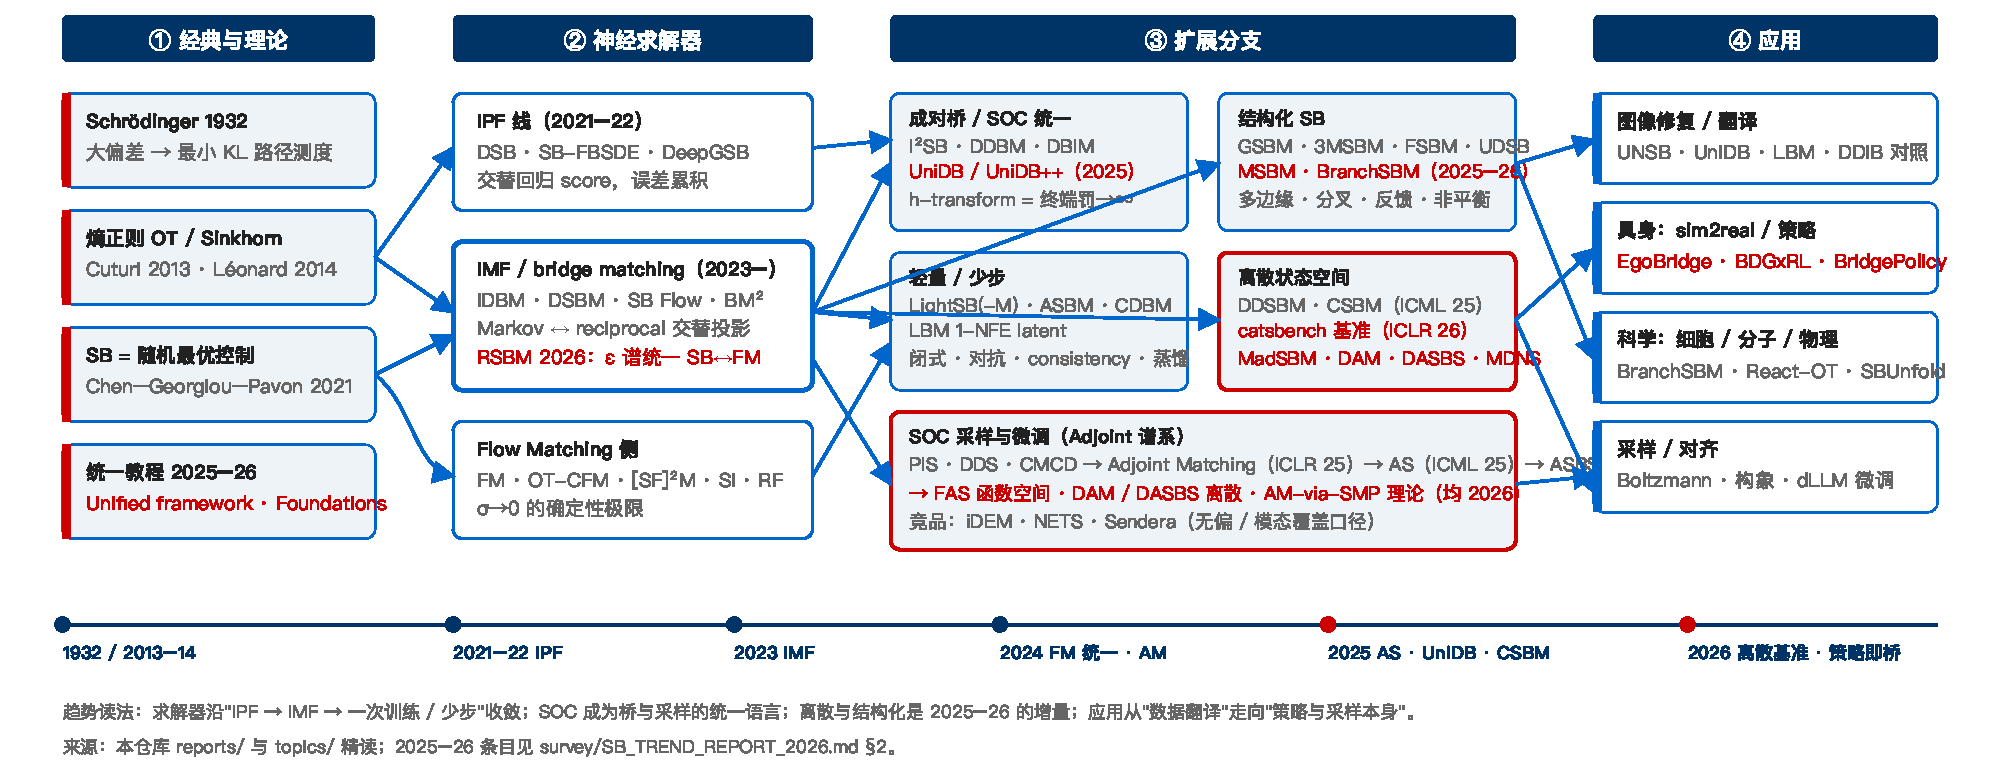
\includegraphics[width=0.98\textwidth]{sb_lineage.pdf}\end{center}
\vspace{-4pt}
{\small 红标 = 2025--2026 新增。求解器沿 IPF $\to$ IMF $\to$ 一次训练 / 少步收敛；SOC 成为桥与采样的统一语言。}
\end{frame}

\section{五条主线}
\begin{frame}{主线 1 · 求解器：IPF $\to$ IMF $\to$ 一次训练与少步}
\begin{columns}[T]
\column{0.48\textwidth}
\textbf{范式切换}
\begin{itemize}
\item DSB（NeurIPS 21）：IPF 交替回归 score，\con{误差累积}
\item DSBM（NeurIPS 23）：IMF 在 Markov / reciprocal 类间交替投影，\pos{两边缘始终保持}
\item SB Flow（NeurIPS 24）：$\alpha$-IMF 在线微调，$\alpha=1$ 退回 IMF
\end{itemize}
\column{0.48\textwidth}
\textbf{$\varepsilon$ 谱与少步}
\begin{itemize}
\item \new{RSBM（2026）}：速度场在 $\varepsilon\in(0,1]$ 上结构不变；3 步 92\% 成功率，3.8$\times$ 更少 NFE
\item CDBM consistency · LBM 1-NFE latent
\item \new{UniDB++}：精确闭式反向解，5--10 步、最多 20$\times$
\end{itemize}
\end{columns}
\vspace{6pt}
\begin{alertblock}{Takeaway}
SB 与 FM 是一条连续谱的两端；同一网络覆盖全谱。缺的是自动选 $\varepsilon$ 的准则。\hfill{\small arXiv:2303.16852 · R:2409.09347 · arXiv:2604.05673 · 2505.21528}
\end{alertblock}
\end{frame}

\begin{frame}{主线 2 · 结构化 SB：把领域知识写进路径}
\vspace{4pt}
\begin{center}\footnotesize\begin{tabular}{P{1.6cm}p{3.9cm}p{5.0cm}p{3.1cm}}\toprule
结构 & 代表 & 关键点 & 证据 \\\midrule
任务代价 & GSBM（ICLR 24） & 路径动能外加可微状态代价 & R:2310.02233 \\\addlinespace[2pt]
多边缘 & 3MSBM · \new{MSBM} & 相空间样条 vs 逐区间局部 SB；两构造并存 & R:2506.10168 · 2510.16587 \\\addlinespace[2pt]
分叉 & \new{BranchSBM（ICLR 26）} & 多速度场 + 增长网络；单分支 SBM 模式塌缩 & ICLR 2026 \\\addlinespace[2pt]
反馈 / 非平衡 & FSBM（ICLR 25 Oral）· UDSB & 闭环反馈控制；质量不守恒 & arXiv:2410.14055 · 2306.09099 \\\addlinespace[2pt]
函数空间 & SOC-FS（NeurIPS 24）$\to$ FAS（ICML 26） & adjoint 采样推到无限维 & R:2511.06239 \\\bottomrule
\end{tabular}\end{center}
\vspace{4pt}
\HL{Takeaway}：结构先验决定生物 / 科学应用能否落地，而不是求解器精度。
\end{frame}

\begin{frame}{主线 3 · 离散状态空间：从翻译到采样与微调}
\begin{columns}[T]
\column{0.48\textwidth}
\textbf{理论与基准}
\begin{itemize}
\item DDSBM（ICLR 25）：CTMC 图变换
\item CSBM（ICML 25）：离散时间 IMF 收敛性
\item \new{catsbench（ICLR 26）}：有解析解的离散分布对 —— 离散 SB 首个 ground truth；副产品 DLightSB(-M)
\end{itemize}
\column{0.48\textwidth}
\textbf{应用 / 微调 / 采样}
\begin{itemize}
\item \new{MadSBM}：肽序列 = 编辑图上的受控 CTMC，参考过程来自 ESM-2 logits
\item \new{DAM（ICLR 26）}：离散 adjoint 估计量，微调 LLaDA-8B
\item \new{DASBS（ICML 26）}：AM 机制与状态空间无关；循环群结构必要
\item \new{MDNS}：CTMC 随机控制训练 masked 扩散采样器
\end{itemize}
\end{columns}
\vspace{6pt}
\HL{Takeaway}：驱动力是 dLLM 与 ground truth；下一步竞争在\textbf{参考过程的选择}。
\end{frame}

\begin{frame}{主线 4 · SOC 采样与微调：Adjoint 谱系的三年}
\begin{itemize}
\item 源头 PIS / DDS / CMCD：全轨迹反传、on-policy 耦合、先验受限（E14）
\item 转折 Adjoint Matching（ICLR 25 Spotlight）：memoryless 调度 + lean adjoint 回归（E06）
\item AS（ICML 25）：梯度更新数 $\gg$ 能量评估数；SPICE 构象 amortized 采样（R:2504.11713）
\item ASBS（NeurIPS 25 Oral）任意 source · FAS 函数空间 · DAM / DASBS 离散
\item 竞品 iDEM / NETS / Sendera：\con{无偏 + 全模态覆盖}仍是短板；评测需补 EUBO / 前向指标（E15）
\item \new{AM via SMP（2026）}：一般 Hamiltonian adjoint matching 目标，一阶变分与 SOC 目标一致；lean adjoint 为状态无关扩散特例
\end{itemize}
\vspace{4pt}
\begin{alertblock}{Takeaway}
Adjoint Matching 把 SOC 变成回归，衍生整条采样 / 微调谱系；2026 年补上了严格数学地基。
\end{alertblock}
\end{frame}

\begin{frame}{主线 5 · 应用面：图像 · 具身 · 科学}
\vspace{4pt}
\begin{center}\footnotesize\begin{tabular}{P{1.9cm}p{6.0cm}p{5.2cm}}\toprule
领域 & 进展 & Takeaway \\\midrule
图像修复 / 翻译 & I²SB $\to$ DDBM $\to$ DBIM $\to$ \new{UniDB / UniDB++}；UNSB、ASBM、LBM 1-NFE & Doob $h$-transform = SOC 终端罚 $\to\infty$ 特例，解释过平滑并给出修法 \\\addlinespace[3pt]
具身 & 表示对齐（EgoBridge、Guided OT）· 生成式 transport（SB Flow、BDGxRL）· \new{策略即桥（BridgePolicy ICML 26、RSBM）} & 三范式不可平替；\con{真机统计协议缺口依旧}（R10 / E11） \\\addlinespace[3pt]
科学 & 单细胞：TrajectoryNet $\to$ DMSB $\to$ 3MSBM $\to$ MSBM $\to$ \new{BranchSBM}；分子：React-OT、AS/ASBS；物理：SBUnfold & 结构化 SB 主战场是单细胞；Adjoint 主战场是构象 \\\bottomrule
\end{tabular}\end{center}
\vspace{2pt}
{\small R:2302.05872 · ICML 2025 · R:2509.19626 · R:2602.23737 · arXiv:2512.07212 · R:2404.13430 · R:2308.12351}
\end{frame}

\section{Insight}
\begin{frame}{Insight I1--I4}
\begin{itemize}
\item \textbf{I1 $\varepsilon$ 是主旋钮}：SB Flow 的 $\alpha$、[SF]$^2$M 的 $\sigma$、RSBM 的 $\varepsilon$、E04 的 $\varepsilon=2\sigma^2$ 说的是同一件事；缺自动选 $\varepsilon$ 的准则（判断）
\item \textbf{I2 SOC 合并了「桥」与「控制」}：UniDB（终端罚 $\to\infty$ = $h$-transform）+ AM（SOC $\to$ 回归）+ SMP（地基）$\Rightarrow$ 设计三元组：参考过程 · 终端罚 · 回归目标
\item \textbf{I3 离散 SB 的两个驱动}：dLLM（DAM / DASBS / MDNS）与 ground truth（catsbench）；下一步在参考过程（MadSBM 用 ESM-2）
\item \textbf{I4 结构先验决定生物应用成败}：多边缘 / 分叉 / 非平衡缺一即塌缩；3MSBM 与 MSBM 两种构造并存，未收敛
\end{itemize}
\vspace{4pt}
{\small 证据：arXiv:2604.05673 · E04 · ICML 2025 · arXiv:2604.08580 · ICLR 2026 · R:2506.10168 · arXiv:2510.16587}
\end{frame}

\begin{frame}{Insight I5--I8}
\begin{itemize}
\item \textbf{I5 具身 SB 进入策略头，评测没跟上}：BridgePolicy / RSBM 的收益来自更好的先验而非更好的翻译；真机统计协议缺口在 2026 年依旧（判断）
\item \textbf{I6 连续高维 SB 仍无 ground truth}：离散有 catsbench，能量采样有 DW4 / LJ / SPICE，unpaired 翻译只有 FID + NFE；coupling 质量需独立指标（E19）
\item \textbf{I7 轻量闭式求解器 = 探针 + 教师}：LightSB(-M) 分钟级 $\varepsilon$ 扫描；DLightSB 搬到离散；LBM / CDBM 说明重模型靠轻模型部署
\item \textbf{I8 开源三簇}：Meta/FAIR（Adjoint 系、flow\_matching、GSBM）· Guan-Horng Liu（SB-FBSDE $\to$ DASBS）· Korotin 组（LightSB 系、ASBM、CSBM、catsbench）
\end{itemize}
\end{frame}

\section{启示与观察}
\begin{frame}{对具身 sim2real 的六条建议}
\begin{enumerate}
\item 先定范式：表示对齐 vs 生成式 transport 不可平替，叠加时分别消融（synthesis §4.4）
\item unpaired 主线以 DSBM-IMF 为基线；同一网络从 $\varepsilon=1$ 走到小 $\varepsilon$ 换 3 步部署（E01 · RSBM）
\item paired 双基线 I²SB + DDBM；用 UniDB 可调终端罚查过平滑（E02 · ICML 25）
\item 任务约束写进 GSBM 状态代价，不做后处理（R:2310.02233）
\item 真机数据极少时试「策略即桥」（判断，需 SimplerEnv 协议验证，E11）
\item 评测先于方法：四层指标 + 功效计算（$\approx$170 rollouts/臂）；coupling 用独立指标；视觉指标服从 policy success
\end{enumerate}
\end{frame}

\begin{frame}{未来 12 个月观察清单}
\vspace{4pt}
\begin{center}\small\begin{tabular}{P{2.6cm}p{6.4cm}p{4.0cm}}\toprule
观察点 & 判据 & 触发动作 \\\midrule
$\varepsilon$ 自动选择 & 自适应 $\varepsilon$ 准则在 unpaired 翻译上验证 & 更新 I1 · README §2.6 \\
连续高维 SB 基准 & catsbench 式解析解基准扩展到连续高维 & 更新 I6 · README §5 \\
dLLM 的 SB/SOC 微调 & DAM / DASBS 之外第二条独立路线，$\ge$7B 验证 & 更新 §2.3 \\
真机统计协议 & 具身 SB 论文报告试次 / 种子 / 置信区间 & 更新 I5 \\
放榜后复核 & 2 条 preprint；FAS / DASBS 页码；MSBM / MadSBM / RSBM / MDNS / AM-SMP venue & 更新 \texttt{metadata/*.tsv} \\\bottomrule
\end{tabular}\end{center}
\end{frame}

\begin{frame}{References（核心与新增）}
\small
\begin{thebibliography}{9}
\bibitem{dsbm} Shi, De Bortoli, Campbell, Doucet. \emph{Diffusion Schrödinger Bridge Matching}. NeurIPS 2023. arXiv:2303.16852.
\bibitem{sbflow} De Bortoli, Korshunova, Mnih, Doucet. \emph{Schrödinger Bridge Flow for Unpaired Data Translation}. NeurIPS 2024. arXiv:2409.09347.
\bibitem{gsbm} Liu, Lipman, Nickel, Karrer, Theodorou, Chen. \emph{Generalized Schrödinger Bridge Matching}. ICLR 2024. arXiv:2310.02233.
\bibitem{am} Domingo-Enrich et al. \emph{Adjoint Matching}. ICLR 2025. arXiv:2409.08861.
\bibitem{asbs} Liu, Choi, Chen, Miller, Chen. \emph{Adjoint Schrödinger Bridge Sampler}. NeurIPS 2025. arXiv:2506.22565.
\bibitem{unidb} Zhu et al. \emph{UniDB: A Unified Diffusion Bridge Framework via SOC}. ICML 2025 (PMLR 267).
\bibitem{branch} Tang, Zhang, Tong, Chatterjee. \emph{Branched Schrödinger Bridge Matching}. ICLR 2026.
\bibitem{cats} Carrasco, Ksenofontov, Leonov, Koshelev, Korotin. \emph{A Benchmark for Schrödinger Bridges and Entropic OT on Discrete Spaces}. ICLR 2026.
\bibitem{bp} \emph{BridgePolicy: Visuomotor Policy Learning via Diffusion Bridge}. ICML 2026. arXiv:2512.07212.
\end{thebibliography}
\end{frame}

\begin{frame}{Thank You}
\begin{center}
{\Large github.com/asimfish/awesome\_Schrodinger\_Bridge}\\[10pt]
加条目：改 \texttt{metadata/extended.tsv} $\to$ \texttt{python3 scripts/build\_readme.py}\\
读精读：\texttt{reports/INDEX.md} · 看趋势：\texttt{survey/SB\_TREND\_REPORT\_2026.md} · 译本 QA：\texttt{papers\_zh/QA\_REPORT.md}\\[10pt]
{\small CC BY 4.0（文本）/ MIT（脚本）· 译本仅供研究学习，引用请以英文原文为准}
\end{center}
\end{frame}

\appendix
\begin{frame}{Backup Slides}\end{frame}
\begin{frame}{Backup · 方法与证据、局限}
\begin{itemize}
\item 来源层次：核心 25 篇逐篇精读（经 10 路审查 + 修复）；专题 20 份；扩展 62 条 = 48 条基础论文（Semantic Scholar 批量核验 47/49，1 条记忆错误剔除）+ 14 条 2026-09-01 新检索（论文页直接可见 ID / 标题 / venue）
\item 未核验即不写：作者不确定留空；venue 无会议页证据写 arXiv；Reflected SBM、CytoBridge 等未能打开原页者未收录
\item 局限：检索日 arXiv API 与 Semantic Scholar 均限流，2025H2--2026 覆盖以 WebSearch 命中为主；数值取自摘要或论文页，未复现
\item 复现：\texttt{build\_readme.py} · \texttt{s2\_verify.py} · \texttt{translate\_batch.sh} · \texttt{qa\_table.py} · \texttt{build\_slides.py} · \texttt{md\_to\_pdf.py}
\end{itemize}
\end{frame}
\begin{frame}{Backup · 术语速查}
\begin{center}\small\begin{tabular}{P{3.2cm}p{9.5cm}}\toprule
术语 & 含义 \\\midrule
SB / EOT & 以参考过程为基准的最小 KL 路径测度 = 动态熵正则 OT \\
IPF / IMF & 交替投影到边缘约束（Sinkhorn 类）/ 交替投影到 Markov 与 reciprocal 类 \\
Bridge matching & 给定端点耦合，回归桥的条件漂移；第一次迭代即合法 transport \\
Doob $h$-transform & 把扩散钉到给定终点的变换；成对桥（I²SB / DDBM）的基础 \\
SOC / Adjoint Matching & 随机最优控制；用 lean adjoint 回归求最优控制，避免全轨迹反传 \\
$\varepsilon$（$\sigma$）谱 & 熵正则强度：$\varepsilon\to 0$ 为确定性 OT / FM，$\varepsilon=1$ 为标准 SB \\\bottomrule
\end{tabular}\end{center}
\end{frame}
\end{document}
